\section{Computational Results}
\label{sec:experiments}

This section evaluates the proposed reformulation and solution method on Tower-derived wireless charging planning instances.
The experiments use the bus network as a realistic source of shared stops, shared links, and route-level service plans, while the main purpose of the section is to validate algorithmic performance.

\subsection{Experimental design and instance families}
\label{subsec:experimental-setup}

The test instances are derived from the Tower Transit bus network in Singapore's Jurong area.
The resulting data set provides a realistic spatial structure with shared stops, shared road links, and multiple routes that may use the same wireless charging infrastructure.
We use these instances as a computational test bed rather than as a public benchmark.

Each scenario represents a plausible future service plan for the same physical network, not random same-day scheduling noise.
Scenario-dependent data include route frequencies, timetables, trip chains, active-fleet requirements, trip-level energy requirements, and charging opportunities induced by the corresponding service plan.
The first-stage wireless charging facilities are shared across all scenarios, whereas route-level battery configurations, charging allocation, and energy management adapt after the service plan is realized.

We use a compact instance code of the form \texttt{N-k}, where \texttt{N} indicates the network scale and $k$ indicates the number of service-plan scenarios.
Specifically, \texttt{S}, \texttt{M}, \texttt{B}, and \texttt{L} denote the small, medium, base, and large Tower-derived networks, respectively.
The capacity-coupling experiment appends \texttt{C}q to the base 10-scenario instance, where $q$ denotes the number of existing plug-in chargers at each plug-in location.
The network-scale family fixes the scenario count at three and varies the physical network scale.
The scenario-count family fixes the base network and varies the number of service-plan scenarios.
Motivated by the relaxation-verification structure in Section~\ref{subsec:route-lower-bounding}, the capacity-coupling family varies plug-in charger capacity on \texttt{B-10} to change how strongly residual plug-in charging demand couples route-level recourse decisions.
Table~\ref{tab:instance-families} summarizes the resulting instance families and their experimental roles.

Travel times are computed from link distances using a nominal operating speed of 30 km/h and then rounded to the one-minute scheduling grid.\footnote{The one-minute lower bound avoids zero-duration movements on short links and absorbs acceleration, deceleration, signal delay, and station-approach time.}
The remaining parameters specify battery costs, charging rates, charging efficiencies, electricity prices, facility costs, and state-of-charge limits.
Table~\ref{tab:parameter-settings} reports the main parameter values used in the computational experiments.

The benchmark ladder consists of five methods: the direct extensive-form MILP, baseline integer L-shaped decomposition, lifted integer L-shaped decomposition, lifted two-phase method, and the full method.
The direct extensive-form MILP optimizes the deterministic equivalent with a commercial solver.
The baseline integer L-shaped decomposition applies the classical scenario decomposition induced by the original two-stage model.
The lifted integer L-shaped decomposition uses the lifted master representation without the two-phase relaxation.
Lifted two-phase adds the Phase 1 lower-bounding and Phase 2 verification structure.
The full implementation further adds tailored Phase 1 cuts and scenario-level monotonicity-strengthened cuts.
Two targeted variants support cut ablations: lifted monotone adds the monotonicity cuts to the lifted single-phase method, while full without Phase 1 custom cuts isolates the effect of monotonicity strengthening under the two-phase framework.

For the decomposition methods, Phase 1 switches at $\varepsilon_1=10^{-4}$ (0.01\%).
Restricted masters and exact scenario MIPs are solved with zero solver gap, and route-level Phase 1 LPs are solved to optimality.
The main performance runs use a 7200-second time limit.

% TODO: Add exact solver version, CPU, memory, thread count, and final outer tolerance epsilon.
% TODO: Add compact size statistics for each instance family after the final data extraction.
% TODO: Add exact statistics for direct MILP on \texttt{B-3} and \texttt{L-3} if those runs are retained.

\begin{figure}[htbp]
    \centering
    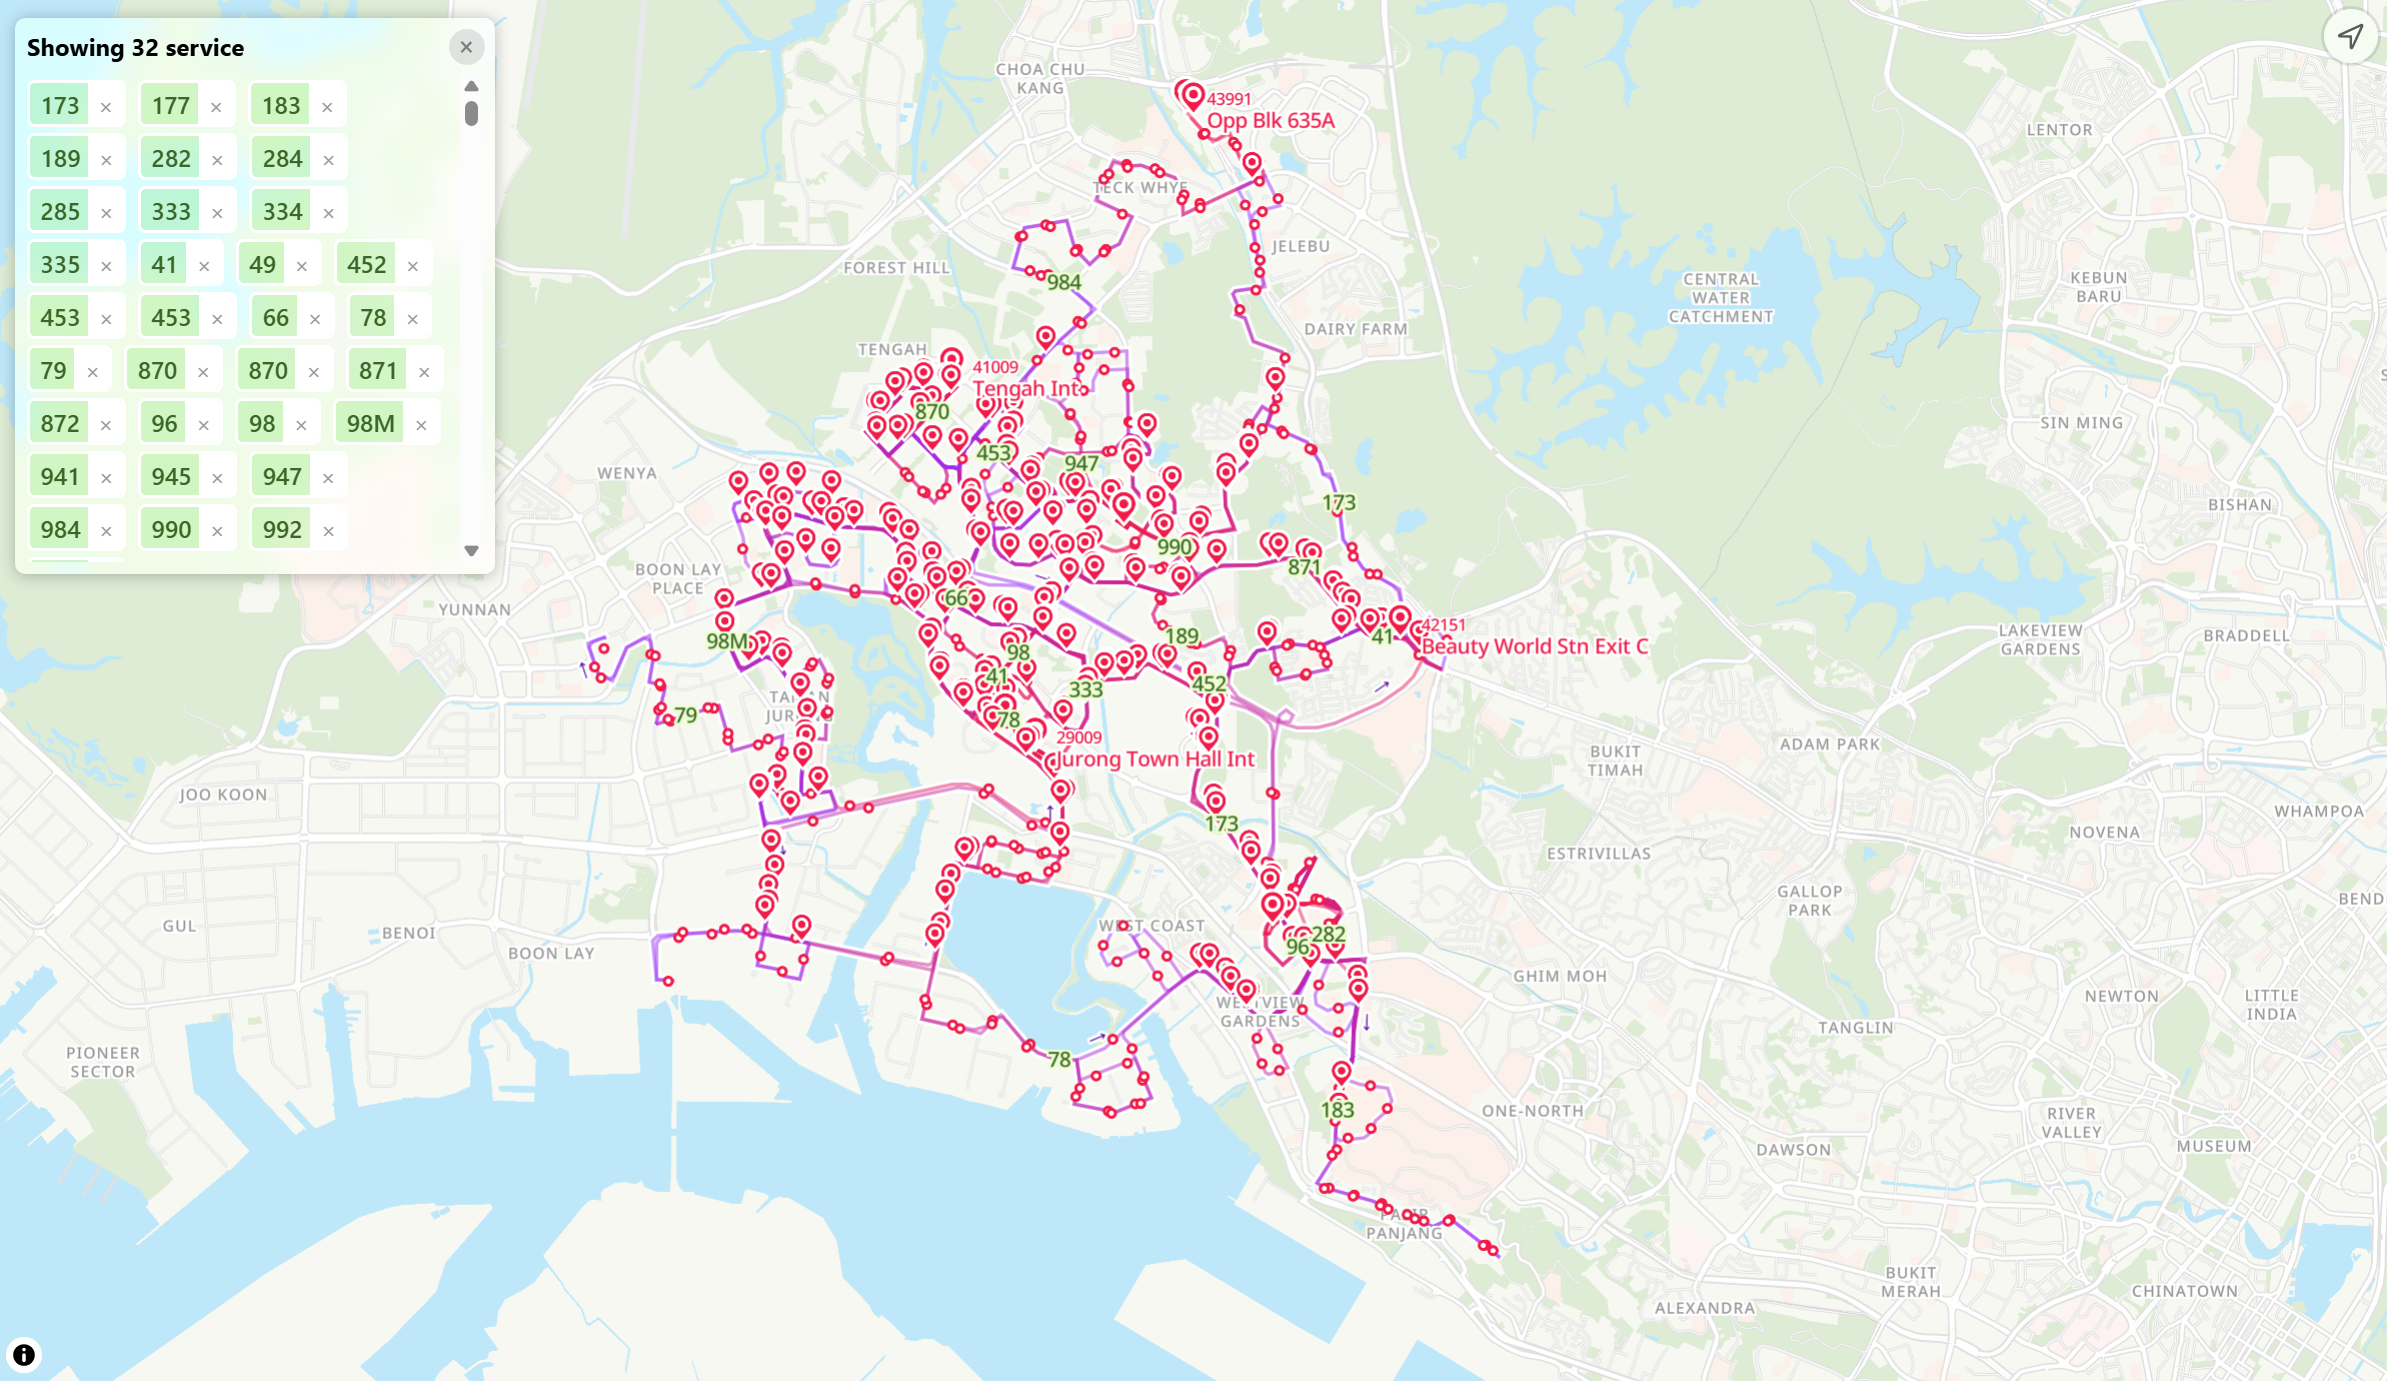
\includegraphics[width=0.88\linewidth]{figures/study_case.png}
    \caption{Spatial layout of the base Tower-derived network in the Jurong area.}
    \label{fig:case-study-map}
\end{figure}

% TODO: Check why the high-frequency scenario has fewer buses than the base scenario in the current generated data.
\begin{table}[htbp]
\centering
\small
\caption{Main instance families and experimental use}
\label{tab:instance-families}
\resizebox{\textwidth}{!}{%
\begin{tabular}{@{}lllll@{}}
\toprule
\textbf{Instance family} & \textbf{Data source or variant} & \textbf{Varied dimension} & \textbf{Primary use} & \textbf{Compared methods} \\
\midrule
\texttt{S-3}, \texttt{M-3}, \texttt{B-3}, \texttt{L-3} & \texttt{tower\_small}, \texttt{tower\_medium}, \texttt{tower}, \texttt{tower\_large} & Network scale, with three scenarios fixed & Network-scale ablation & Direct MILP, baseline integer L-shaped, lifted integer L-shaped, lifted two-phase, full method \\
\texttt{B-}k, $k\in\{3,5,10,20,40\}$ & \texttt{tower}, \texttt{tower\_5}, \texttt{tower\_10}, \texttt{tower\_20}, \texttt{tower\_40} & Scenario count, with base network fixed & Scenario-count scalability & Full method \\
\texttt{B-10-C}q, $q\in\{2,3,4,5,6\}$ & Capacity variants of \texttt{tower\_10} & Existing plug-in charger units, with base network and 10 scenarios fixed & Relaxation-gap stress test & Full method \\
\bottomrule
\multicolumn{5}{@{}l}{\footnotesize \texttt{B-3} is the representative base instance used for solution interpretation; larger $q$ indicates more existing plug-in charger units.} \\
\end{tabular}
}
\end{table}

\begin{table}[htbp]
\centering
\small
\caption{Parameter settings for the computational experiments}
\label{tab:parameter-settings}
\resizebox{\textwidth}{!}{%
\begin{tabular}{@{}>{\raggedright\arraybackslash}p{0.16\linewidth}>{\raggedright\arraybackslash}p{0.30\linewidth}>{\raggedright\arraybackslash}p{0.18\linewidth}>{\raggedright\arraybackslash}p{0.28\linewidth}@{}}
\toprule
\textbf{Parameter} & \textbf{Description} & \textbf{Value} & \textbf{Source} \\
\midrule
\multicolumn{4}{@{}l}{\textit{Battery and state of charge}} \\
$c^{\mathrm{bat}}$ & Daily-equivalent battery capacity cost & 0.148 USD/kWh/day & BloombergNEF price amortized over Wang et al. battery life \citep{bloombergnef_lithium-ion_2025,wang_reliable_2024} \\
$\mathcal{K}$ & Candidate route-level battery options & 10-kWh increments within instance bounds & Case-data preprocessing \\
$\underline{\rho},\overline{\rho}$ & Minimum and maximum state-of-charge fractions & 0.2, 0.8 & Wireless bus planning literature \citep{li_planning_2024} \\
\addlinespace
\multicolumn{4}{@{}l}{\textit{Charging operation}} \\
$\kappa$ & Maximum plug-in energy per occupied one-minute slot & 2.5 kWh/slot & \citet{najafi_integrated_2025} \\
$\bar q_v^{\mathrm{S}}$ & Visit-specific SWC opportunity limit & 1.0 kWh/min times eligible dwell time & \citet{wang_reliable_2024} \\
$\bar q_a^{\mathrm{D}}$ & Traversal-specific DWC opportunity limit & 1.0 kWh/min times traversal time & \citet{wang_reliable_2024} \\
$\eta^{\mathrm{P}}$ & Plug-in charging efficiency & 0.90 & \citet{li_planning_2024} \\
$\eta^{\mathrm{S}}$ & Stationary wireless charging efficiency & 0.85 & \citet{sun_optimizing_2024} \\
$\eta^{\mathrm{D}}$ & Dynamic wireless charging efficiency & 0.80 & \citet{sun_optimizing_2024} \\
$U_s$ & Existing plug-in charger units at plug-in location $s$ & 4 chargers in the base setting & Case-study assumption \\
\addlinespace
\multicolumn{4}{@{}l}{\textit{Infrastructure and electricity cost}} \\
$T^{\mathrm{fac}}$ & Facility amortization horizon & 30 years & \citet{wang_reliable_2024} \\
$c_s^{\mathrm{S}}$ & Daily-equivalent cost of an SWC facility & 2.16 USD/day & \citet{wang_reliable_2024} \\
$c_l^{\mathrm{D}}$ & Daily-equivalent cost of a DWC facility on link $l$ & 9 USD/km/day times link length, plus 0.90 USD/day & \citet{wang_reliable_2024} \\
$c^{\mathrm{day}}$ & Daytime electricity price & 0.1922 USD/kWh & Singapore tariff data \citep{singstat_electricity_2026} \\
$c^{\mathrm{night}}$ & Nighttime electricity price & 0.1233 USD/kWh & Singapore tariff data \citep{singstat_electricity_2026} \\
\bottomrule
\end{tabular}
}
\end{table}

\subsection{Solution characteristics on the base Tower instance}
\label{subsec:solution-characteristics}

This subsection will use the full-method solution for \texttt{B-3} to examine whether the optimized plan is interpretable at the facility, battery, and charging levels.
Table~\ref{tab:planned-solution-summary} lists the outputs to be reported once the final decision data are extracted.

\begin{table}[htbp]
\centering
\small
\caption{Planned summary of the representative \texttt{B-3} solution}
\label{tab:planned-solution-summary}
\begin{tabular}{@{}>{\raggedright\arraybackslash}p{0.22\linewidth}>{\raggedright\arraybackslash}p{0.36\linewidth}>{\raggedright\arraybackslash}p{0.34\linewidth}@{}}
\toprule
\textbf{Result block} & \textbf{Reported quantities} & \textbf{Purpose} \\
\midrule
Cost composition & Facility, expected battery, daytime charging, and overnight charging costs & Verify how the objective is distributed across planning and recourse decisions \\
Facility deployment & Numbers of selected SWC stations and DWC links, together with representative selected locations & Identify where the optimized layout creates charging opportunities \\
Battery adaptation & Route-level battery capacities by scenario and their minimum, median, and maximum values & Show how battery configurations adapt across service plans \\
Charging allocation & Plug-in, SWC, DWC, and overnight charging energy, plus peak plug-in utilization & Describe how wireless deployment and shared plug-in capacity interact \\
\bottomrule
\end{tabular}
\end{table}

A second compact table will list representative selected stations or links, their facility type, and the routes and scenarios that use them.
The accompanying analysis will distinguish shared network-level deployments from route-specific charging opportunities and will relate the selected battery capacities to residual plug-in charging demand.

% TODO: Populate both solution-characteristics tables after extracting the final B-3 decisions.

\subsection{Network-scale algorithmic ablation}
\label{subsec:network-scale-results}

The network-scale ablation fixes the number of service-plan scenarios at three and increases the physical network size from \texttt{S-3} to \texttt{L-3}.
Table~\ref{tab:network-ablation} reports the available runs across the core benchmark ladder and tracks how the solvable boundary changes as the lifted and two-phase components are introduced.

\begin{table}[htbp]
\centering
\small
\caption{Network-scale ablation under three service-plan scenarios}
\label{tab:network-ablation}
\resizebox{\textwidth}{!}{%
\begin{tabular}{@{}lccccc@{}}
\toprule
\textbf{Instance} & \textbf{Direct MILP} & \textbf{Baseline integer L-shaped} & \textbf{Lifted integer L-shaped} & \textbf{Lifted two-phase} & \textbf{Full method} \\
\midrule
\texttt{S-3} & Opt., 4.2s & TL, 98.37\% & TL, 77.84\% & Opt., 0.4s & Opt., 0.4s \\
\texttt{M-3} & TL, 0.27\% & n.r. & n.r. & Opt., 25.8s & Opt., 25.7s \\
\texttt{B-3} & n.r. & n.r. & n.r. & Opt., 29.4s & Opt., 32.2s \\
\texttt{L-3} & n.r. & n.r. & n.r. & TL, 0.092\% & TL, 0.092\% \\
\bottomrule
\multicolumn{6}{@{}l}{\footnotesize Opt. = reached the prescribed optimality tolerance; TL = 7200s time limit; n.r. = not reported in the current run set.} \\
\multicolumn{6}{@{}l}{\footnotesize Percentages are final relative gaps at termination.} \\
\end{tabular}
}
\end{table}

The results identify the two-phase structure as the main computational transition in this run set.
On \texttt{S-3}, the direct MILP is still easy, but the standard integer L-shaped variants make little progress within the time limit because their master lower bounds remain weak.
Once route-level lower bounding and exact Phase 2 verification are introduced, both two-phase variants solve \texttt{S-3}, \texttt{M-3}, and \texttt{B-3}.
Both two-phase variants reach the time limit on \texttt{L-3}; Table~\ref{tab:mechanism-contrast} reports their terminal bounds.

\begin{table}[htbp]
\centering
\small
\caption{Two-phase boundary diagnostics on the largest three-scenario instance}
\label{tab:mechanism-contrast}
\begin{tabular}{@{}lrrrrr@{}}
\toprule
\textbf{Method} & \textbf{Status} & \textbf{UB} & \textbf{LB} & \textbf{Gap (\%)} & \textbf{Time (s)} \\
\midrule
Lifted two-phase & TL & 27251.656 & 27226.537 & 0.092 & 7217.5 \\
Full method & TL & 27251.656 & 27226.537 & 0.092 & 7231.9 \\
\bottomrule
\multicolumn{6}{@{}l}{\footnotesize Both runs stop during Phase 2.} \\
\end{tabular}
\end{table}

The identical terminal bounds place the current network-scale boundary between \texttt{B-3} and \texttt{L-3} and show no additional benefit from the full-method enhancements on this instance.
Exact Phase 2 verification remains the limiting operation at this scale.

\subsection{Scenario-count scalability}
\label{subsec:scenario-scale-results}

This subsection uses the \texttt{B-}k family, with $k\in\{3,5,10,20,40\}$, to test scenario-count scalability on the base Tower-derived network.
To isolate growth in the scenario dimension while holding the network and algorithm fixed, Table~\ref{tab:scenario-scalability} reports the full method and separates Phase 1 and Phase 2 time.

\begin{table}[htbp]
\centering
\small
\caption{Scenario-count scalability on the base Tower-derived network}
\label{tab:scenario-scalability}
\resizebox{\textwidth}{!}{%
\begin{tabular}{@{}lrrrrrr@{}}
\toprule
\textbf{Instance} & \textbf{UB} & \textbf{LB} & \textbf{Gap (\%)} & \textbf{P1 time (s)} & \textbf{P2 time (s)} & \textbf{Total (s)} \\
\midrule
\texttt{B-3}  & 7869.832 & 7869.814 & 0.000 & 19.2 & 13.1 & 32.2 \\
\texttt{B-5}  & 7852.604 & 7852.340 & 0.003 & 27.4 & 30.3 & 57.7 \\
\texttt{B-10} & 7862.021 & 7861.809 & 0.003 & 59.0 & 60.6 & 119.7 \\
\texttt{B-20} & 7850.547 & 7850.375 & 0.002 & 126.6 & 120.8 & 247.4 \\
\texttt{B-40} & 7849.108 & 7848.937 & 0.002 & 345.5 & 580.9 & 926.4 \\
\bottomrule
\multicolumn{7}{@{}l}{\footnotesize All five runs converge within the prescribed tolerance; reported times are wall-clock seconds.} \\
\end{tabular}
}
\end{table}

The full method solves all tested scenario counts within the prescribed tolerance.
Total solution time increases from 32.2 seconds for \texttt{B-3} to 926.4 seconds for \texttt{B-40}, while all final gaps remain below 0.004\%.
Both phases grow with the scenario count, and Phase 2 becomes the larger time component at 40 scenarios because each master candidate requires more exact scenario evaluations.

\subsection{Capacity-coupling and relaxation-gap stress test}
\label{subsec:capacity-coupling-results}

This subsection uses \texttt{B-10-C2} through \texttt{B-10-C6} to test the effect of shared plug-in charger capacity on the relaxation-verification structure.
All five variants are built from \texttt{B-10}; only the number of existing plug-in chargers is varied.
Tighter capacity increases cross-route competition that is absent from the Phase 1 relaxation in Proposition~\ref{prop:phase-one-lb}, whereas looser capacity should bring the relaxed and exact recourse problems closer.
Table~\ref{tab:capacity-coupling} reports the full method only and uses the initial Phase 2 gap as a transition diagnostic for the complete algorithm.

\begin{table}[htbp]
\centering
\small
\caption{Capacity-coupling and relaxation-gap stress test on \texttt{B-10}}
\label{tab:capacity-coupling}
\resizebox{\textwidth}{!}{%
\begin{tabular}{@{}lrrrrrr@{}}
\toprule
\textbf{Instance} & \textbf{Status} & \textbf{UB} & \textbf{LB} & \textbf{Final gap (\%)} & \textbf{Initial P2 gap (\%)} & \textbf{Total (s)} \\
\midrule
\texttt{C2} & TL & -- & -- & -- & -- & 7243.1 \\
\texttt{C3} & Opt. & 7871.295 & 7870.696 & 0.008 & 0.676 & 280.5 \\
\texttt{C4} & Opt. & 7862.021 & 7861.809 & 0.003 & 0.562 & 148.2 \\
\texttt{C5} & Opt. & 7859.664 & 7859.497 & 0.002 & 0.532 & 95.9 \\
\texttt{C6} & Opt. & 7859.271 & 7859.164 & 0.001 & 0.527 & 114.0 \\
\bottomrule
\multicolumn{7}{@{}l}{\footnotesize \texttt{C}q denotes $q$ existing plug-in chargers at each plug-in charging location. \texttt{C2} reaches the Phase 2 time limit before a verified objective pair is recorded.} \\
\end{tabular}
}
\end{table}

As plug-in capacity increases from \texttt{C3} to \texttt{C6}, the initial Phase 2 gap falls from 0.676\% to 0.527\%, and the final optimality gaps after convergence remain below 0.008\%.
The tightest reported setting, \texttt{C2}, is qualitatively different: Phase 1 still solves the relaxed problem quickly, but Phase 2 repeatedly separates feasibility cuts and reaches the time limit.
Thus, the complete method handles the tested \texttt{C3}--\texttt{C6} range, while \texttt{C2} exposes a clear limitation: sufficiently tight shared capacity can make exact verification the computational bottleneck.
